\section{Enquadramento técnico-científico e análise crítica}
\orientacao{Apresentar, discutir e analisar criticamente os conceitos, fundamentos, conhecimentos, soluções, metodologias, tecnologias ou práticas relevantes para o trabalho, sustentando a discussão em fontes bibliográficas relevantes e credíveis. Identificar, quando aplicável, vantagens, limitações, lacunas e oportunidades, fundamentando o posicionamento do trabalho a desenvolver.}
\orientacao{Organizar o conteúdo em secções e/ou subsecções temáticas, de acordo com a natureza e a especificidade da D/P/E. A análise crítica e o posicionamento do trabalho poderão ser desenvolvidos de forma integrada ou em secções autónomas, consoante a organização considerada mais adequada pelo estudante.}

Lorem ipsum dolor sit amet, consectetur adipiscing elit. Sed do eiusmod tempor incididunt ut labore et dolore magna aliqua. Ut enim ad minim veniam, quis nostrud exercitation ullamco laboris nisi ut aliquip ex ea commodo consequat. Duis aute irure dolor in reprehenderit in voluptate velit esse cillum dolore eu fugiat nulla pariatur.


% Exemplo de equação: eliminar ou adaptar na versão de entrega.
\orientacao{Quando aplicável, as equações deverão ser numeradas, referenciadas no texto e acompanhadas da identificação das grandezas e parâmetros envolvidos. O exemplo seguinte é meramente ilustrativo; a inclusão de equações não é obrigatória.}
\orientacao{A Equação~\eqref{eq:hooke} representa a lei de Hooke no regime elástico linear uniaxial.}
\begin{equation}
  \sigma = E\varepsilon
  \label{eq:hooke}
\end{equation}
\orientacao{Nesta expressão, $\sigma$ representa a tensão normal, $E$ o módulo de Young e $\varepsilon$ a deformação longitudinal.}

% Exemplo de figura: eliminar ou substituir na versão de entrega.
\orientacao{Todas as figuras devem ser referidas no texto e acompanhadas de uma legenda descritiva, indicando a fonte quando aplicável. A Figura~\ref{fig:T2fig} apresenta um exemplo de inserção e referenciação de uma figura.}
\begin{figure}[!htb]
\centering
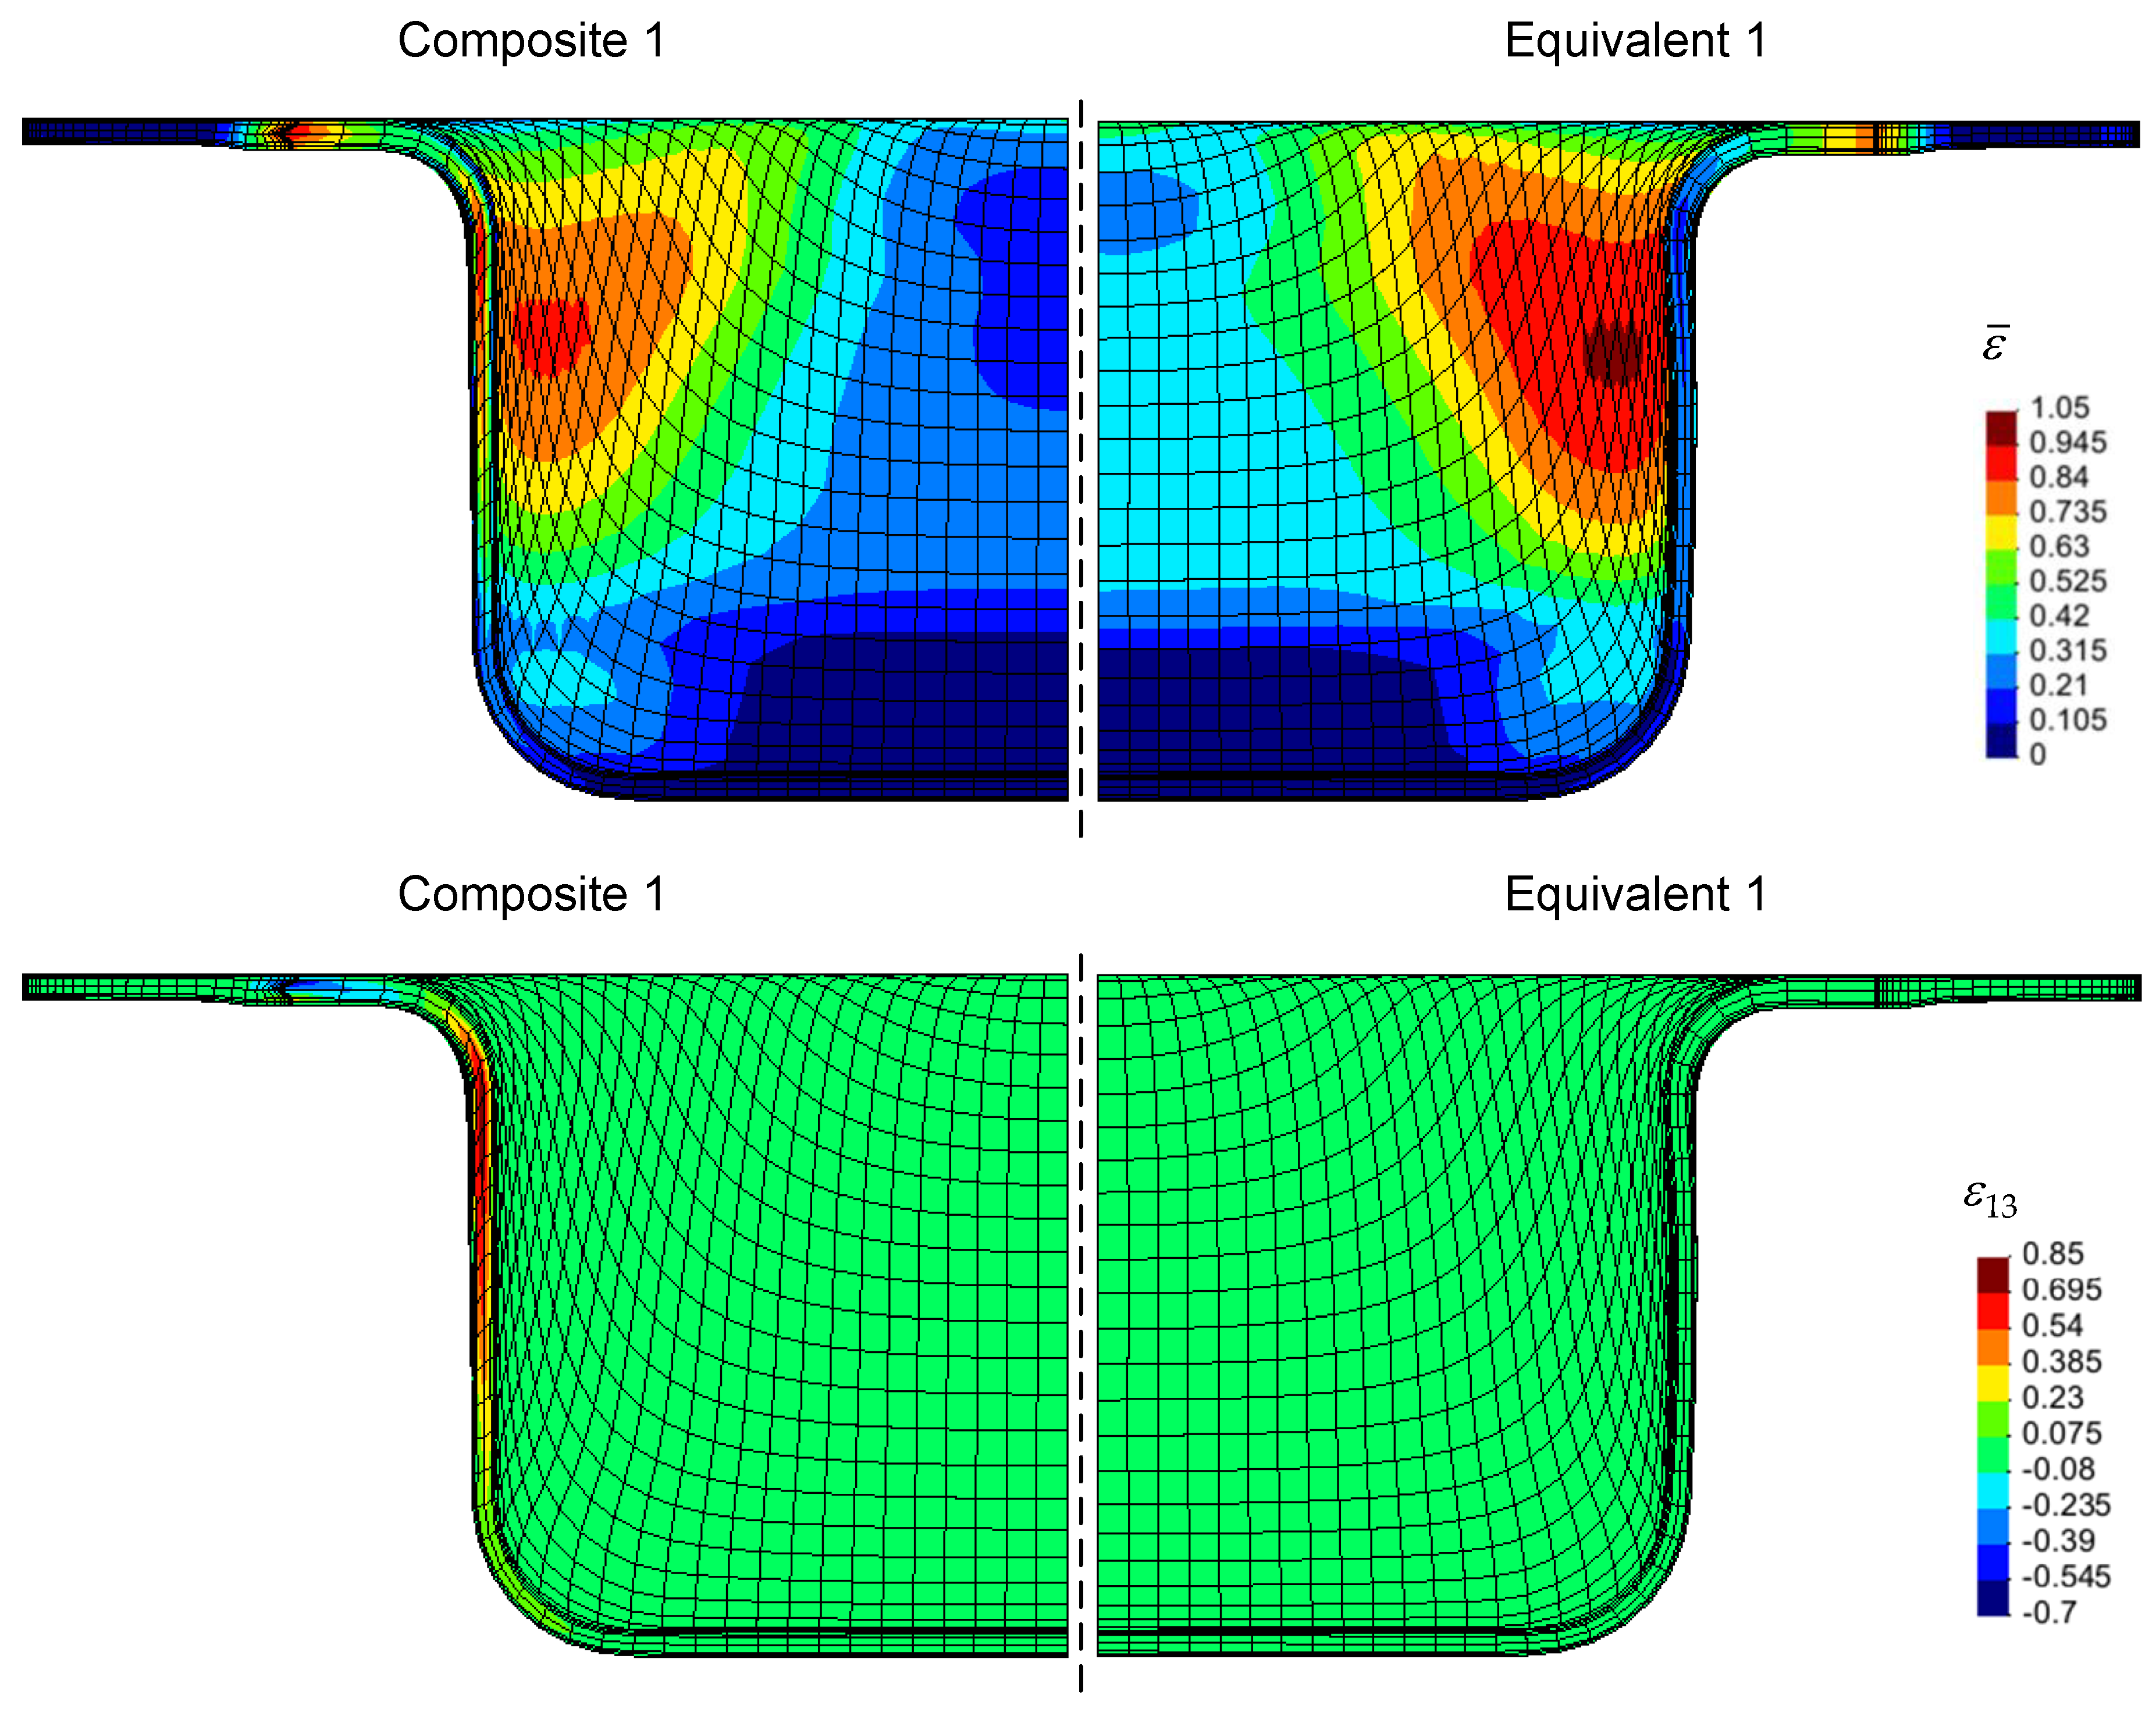
\includegraphics[width=0.65\linewidth]{pics/Fig1.png}
\caption{Exemplo de figura 1.}
\label{fig:T2fig}
\end{figure}
\orientacao{A Tabela~\ref{tab:exemplo} exemplifica a comparação crítica da literatura. A tabela é meramente exemplificativa, tanto na sua estrutura como no seu conteúdo. A utilização de tabelas de síntese ou de análise comparativa e a definição dos respetivos critérios deverão ser adequadas à natureza do tema e aos objetivos da revisão. Caso seja utilizada, deverá basear-se em trabalhos efetivamente consultados e citados. As legendas das tabelas devem ser colocadas acima das mesmas.}
\begin{table}[!htb]
\centering
\caption{Exemplo ilustrativo de uma tabela de análise comparativa da literatura.}
\label{tab:exemplo}
\normalsize
\renewcommand{\arraystretch}{1.2}
\begin{tabularx}{\linewidth}{@{}*{4}{>{\raggedright\arraybackslash}X}@{}}
\toprule
\textbf{Referência} & \textbf{Metodologia} & \textbf{Principais contributos} & \textbf{Limitações} \\
\midrule
Estudo A & Modelação analítica & Reduzido custo computacional & Hipóteses simplificativas \\
Estudo B & Simulação numérica & Flexibilidade de aplicação & Elevado custo computacional \\
Estudo C & Abordagem experimental & Validação em condições reais & Aplicabilidade limitada \\
\bottomrule
\end{tabularx}
\end{table}

\clearpage